Now that we've understood that the $-1/x^2$ potential could have something different from the other ones, let's investigate some of its peculiarities following the procedure that has been done by Essin and Griffiths~\cite{EssinGriffiths:10.1119/1.2165248}.

First consider the explicit form of the potential we're going to examine:

\begin{equation*}
    V(x) = \begin{cases}
        \infty    & \text{if } x \leq 0 \\
        - a / x^2 & \text{if } x > 0
    \end{cases}
\end{equation*}

which is shown in Figure~\ref{fig:potential}.

\subsection*{The dimensional problem}

Even though we haven't done anything yet, there is already something worth noticing. In fact, from the parameters present in our problem, \textit{i.e. \(\hbar\), \(m\), and \(a\)}, there is no way to construct a quantity with the dimensions of energy.

Let's show it from the dimensional analysis. Our parameters have the following dimension:

\begin{align*}
    [\hbar] = E \cdot T, \quad [m] = E \cdot T^2 \cdot L^{-2}, \quad [a] = E \cdot L^2.
\end{align*}

\noindent
So we want to look for three parameters $\alpha$,$\beta$ and $\delta$ that satisfy

\begin{align*}
    E & = \hbar^\alpha m^\beta a^\delta                                                      \\
      & = (E \cdot T)^\alpha (E \cdot T^2 \cdot L^{-2})^\beta (E \cdot L^2)^\delta           \\
      & = E^{\alpha + \beta + \delta} \cdot T^{\alpha + 2\beta} \cdot L^{-2\beta + 2\delta}.
\end{align*}

\noindent
So we are lead to an equation for each quantity, \textit{i.e. the system}:

\begin{align*}
    \begin{cases}
        E: & 1 = \alpha + \beta + \delta \\
        T: & 0 = \alpha + 2\beta         \\
        L: & 0 = -2\beta + 2\delta
    \end{cases}
    \quad
    \begin{cases}
        1 = - 2\beta + \beta + \beta \\
        \alpha = -2\beta             \\
        \delta = \beta
    \end{cases}
    \quad
    \begin{cases}
        1 = 0            \\
        \alpha = -2\beta \\
        \delta = \beta
    \end{cases}
\end{align*}

\noindent
Se we have no solutions, hence no possible formula for the eigenvalues of the Hamiltonian.
The issue will be resolved when we use the mathematical method of self-adjoint extension on our Hamiltonian to make it an Observable. A new parameter will be introduced, and by using it, the dimensional problem of the eigenvalue formula disappears.
We'll se in the Section \ref{section:delta_potential} that this properties is not unique of this potential.

\begin{figure}
    \centering
    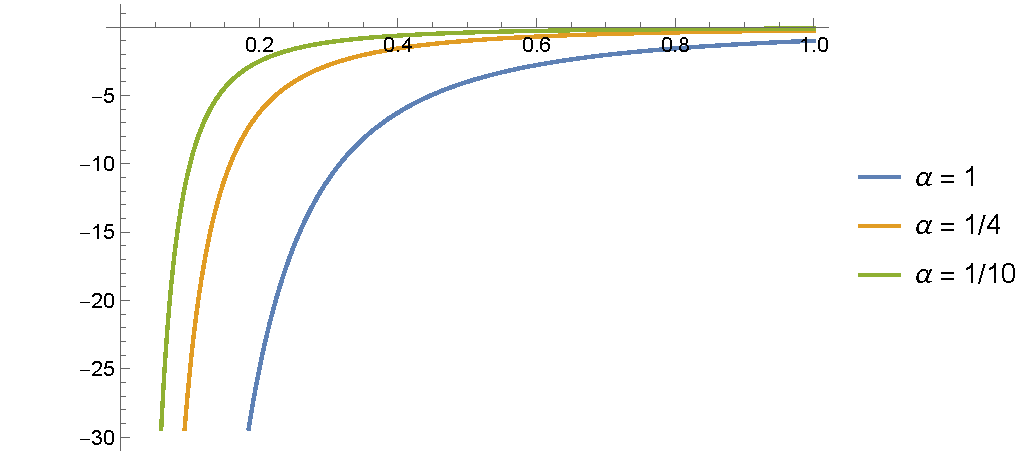
\includegraphics[width=0.8\linewidth]{potential.pdf}
    \caption{The $-\alpha/x^2$ function.}
    \label{fig:potential}
\end{figure}

\vspace{4mm}
\noindent
Let's pretend that we haven't noticed the problem. We're looking for bounded energy states (\textit{i.e. \(E < 0\)}) that are normalized and solutions of the Schrödinger equation:
\begin{align}
    - \frac{\hbar^2}{2m} \frac{d^2\psi}{dx^2} - \frac{a}{x^2}\psi = E \psi
    \label{eq:eigenvalue_boundstate}
\end{align}

where the naive boundary condition are
\begin{align*}
    \lim_{x \to 0} \psi = 0 \quad \text{and} \quad \lim_{x \to +\infty} \psi = 0
\end{align*}

\noindent
Since our intuition leads us to require the wave function to be zero on the negative half-axis and continuous, as well as square-integrable.
\footnote{The latter condition exclude some pathological cases of square integrable functions that does not converge at infinity such $f(x) = x^2 e^{-x^8 \sin^2(x)}$.}

\subsection{The scale invariance symmetry}
Keeping in mind what we have build until now, we want to show the symmetry of our problem on the half-axis, that is the scale invariance and then we want to show what does it imply.

So suppose we found a bound state $\psi(x)$ (\textit{i.e. $E<0$}), that means it satisfies the Equation~\eqref{eq:eigenvalue_boundstate}.

Scaling the variable $x$ by a factor $\beta$, we can easily construct a new solution $\psi_\beta (x) := \psi (\beta x)$ with energy $\beta^2 E$:
\begin{align*}
    H \psi_\beta
     & = - \frac{\hbar^2}{2m} \frac{d^2}{dx^2}\psi_\beta(x) - \frac{a}{x^2} \psi_\beta(x)                                  \\
     & = - \frac{\hbar^2}{2m} \frac{d^2}{dx^2}\psi(\beta x) - \frac{a}{x^2} \psi(\beta x)                                  \\
     & = - \beta^2 \frac{\hbar^2}{2m} \frac{d^2}{d(\beta x)^2} \psi(\beta x) - \beta^2 \frac{a}{(\beta x)^2} \psi(\beta x) \\
     & = - \beta^2 \left(\frac{\hbar^2}{2m} \frac{d^2}{d(\beta x)^2} - \frac{a}{(\beta x)^2}\right) \psi(\beta x) \\
     & = \beta^2 E \, \psi_\beta (x)
\end{align*}
Since $\beta \in \mathbb{R}$ is arbitrary, we can construct an eigenfunction for each negative eigenvalue (remember that we supposed the existence of a bound state). That means that the lowest energy level is $E = -\infty$ (\textit{i.e. it doesn't exist}).

So we can conclude that if a problem is scale invariant, it cannot admit a ground state.\footnote{The absence of the ground state that we've just derived will turn out to be an indication of the inconsistency of the problem we've introduced with Quantum Mechanics, as we will reach a different conclusion in Section~\ref{section:xsqared_halfaxis}.}

\vspace{4mm}
\noindent
What we have learned from the scale invariance is that for every $a$ the $-a/x^2$ potential has no ground state and the allowed energies for bounded states (if they exist) are not quantized, but we can discuss if the value of $a$ has relevance in the existence of a bound state.

First, let's rewrite our problem to make its mathematical aspects clearer: by multiplying Eq.~\eqref{eq:eigenvalue_boundstate} by $2m/\hbar^2$, we obtain:
\footnote{We conventionally use \(\rho\) for bound states and \(k\) for scattering states.}
\begin{align}
    - \frac{d^2\psi}{dx^2} - \frac{\alpha}{x^2}\psi = - \rho^2 \psi, \quad  -\rho^2 := \frac{2mE}{\hbar^2}, \quad \alpha := \frac{2ma}{\hbar^2}.
    \label{eq:eigenvalue_boundstate_alpha}
\end{align}

\subsubsection{Case: \(\alpha < 0\)}
Obviously, since in this situation the potential becomes repulsive, bound states are forbidden.

\subsubsection{Case: \(\alpha < 1/4\)}

To show some properties of this case it's convenient to define $\nu \, (1-\nu) := \alpha$, and then rewrite our Hamiltonian as follow:
\begin{align*}
    H & = - \frac{\hbar^2}{2m} \left(\frac{d^2}{dx^2} + \frac{\alpha}{x^2}\right) \\
      & = - \frac{\hbar^2}{2m} \left( \frac{d}{dx} + \frac{\nu}{x} \right) \left( \frac{d}{dx} - \frac{\nu}{x} \right) = - \frac{\hbar^2}{2m} A B
\end{align*}
Where we defined $A$ and $ B $ respectively as the two differential operators in the parenthesis.

Let show its correctness acting of a test function $f(x)$:
\begin{align*}
    A B f
     & = A \left( \frac{d}{dx} - \frac{\nu}{x} \right) f                                     \\
     & = A \left( f' - \frac{\nu}{x} f \right)                                               \\
     & = \left( \frac{d}{dx} + \frac{\nu}{x} \right) \left( f' - \frac{\nu}{x}f \right)      \\
     & = f'' + \frac{\nu}{x^2} f - \frac{\nu}{x} f' + \frac{\nu}{x} f' - \frac{\nu^2}{x^2} f \\
     & = f'' + \frac{\nu \, (1-\nu)}{x^2} f                                                  \\
     & = \left( \frac{d^2}{dx^2} + \frac{\alpha}{x^2} \right) f .
\end{align*}

\noindent
Before the next step it's useful to notice that $A^\dagger = - B^*$:

\begin{align*}
    \langle f | A g \rangle
     & = \int_{0}^{\infty} f^* \left( \frac{d}{dx} + \frac{\nu}{x} \right) g                                                            \\
     & = f^* g \Big|_0^\infty - \int_{0}^{\infty}  \left[\left( \frac{df}{dx} \right)^* g + \left( \frac{\nu^* f}{x} \right)^* g\right] \\
     & = - \int_{0}^{\infty} \left( \frac{df}{dx} - \frac{\nu^* f}{x} \right)^* g                                                       \\
     & = - \langle B^* f |  g \rangle
\end{align*}

provided that $f$ and $g$ vanish at zero and infinity.

\vspace{4mm}
\noindent
So now we can obtain a formula for the energy of a given state $\psi$ using $A$ and $B$:
\begin{align*}
    E & = \langle \psi | H \psi \rangle             \\
      & = - \frac{\hbar^2}{2m} \langle \psi | A B \psi \rangle         \\
      & = - \frac{\hbar^2}{2m} \langle A^\dagger \psi | B \psi \rangle \\
      & = \frac{\hbar^2}{2m} \langle B^* \psi | B \psi \rangle
\end{align*}
That means if $\nu$ is real, then $B^* = B$, and as a result, $E = (\hbar^2/2m) || B \psi ||^2$, which is strictly greater than zero. Therefore, we have concluded that the realness of $\nu$ precludes the existence of negative energy states (\textit{i.e. no bound states}).\footnote{This result will be shown to be incorrect in Section~\ref{section:xsqared_halfaxis}. The cause of this discrepancy lies in the fact that, with the correct boundary conditions, the boundary term does not vanish.}
This condition, since
\begin{equation*}
    \nu = \frac{1}{2} \pm \sqrt{\frac{1}{4} - \alpha}
\end{equation*}

is equivalent to the condition $\alpha < 1/4$.

\subsubsection{Case: \(\alpha > 1/4\)}

This case imply that $\nu$ is not purely real, so the existence of bound state is not forbidden. Let's look for the bound state trough the Frobenius method, so writing $\psi(x)$ as the following power series
\begin{align*}
    \psi(x) = x^s \sum_{j=0}^{\infty} a_j x^j \quad a_0 \neq 0
\end{align*}

and substituting in the Schrodinger equation \eqref{eq:eigenvalue_boundstate}, we obtain (multiplying by $-1/x^s$)
\begin{align*}
    \sum_{j=0}^{\infty} a_j [(j+s)(j+s-1) + \alpha] x^{j-2} = \rho^2 \sum_{j=0}^{\infty} a_j x^j
\end{align*}
Which, since $a_0 \neq 0$, for the $1/x^2$ term yields $s(s-1)+\alpha = 0$ (\textit{i.e. $s = \nu$}), while fot the $1/x$ term yields $a_1 [(1+s)s + \alpha] = 0$. Using the relation between $\alpha$ and $s$ the equation becomes $a_1 2 s = 0$, but since $s$ is already determined, $a_1 = 0$.

The remaining coefficient are determined by recursion, we can show it changing variable in the left sum: $l + 2 = j$
\begin{align*}
    \sum_{l=0}^{\infty} a_{l+2} [(l+2+s)(l+s+1) + s(1-s)] x^{l} = \rho^2 \sum_{j=0}^{\infty} a_j x^j
\end{align*}

rewriting $(l+2+s)(l+s+1) + s(1-s) $ and equate like powers, so we obtain:
\begin{align*}
    a_{j+2} = \frac{\rho^2}{(2+l)(1+l+2s)} a_j \quad j \in \mathbb{N}
\end{align*}

\noindent
Now remembering that $s$ has two solutions (like $\nu$), from now on called $s_\pm$, $\psi(x)$ will have two solutions too (remember also that we're solving a second order differential equation). Those solutions behave near the origin in the following way
\begin{align*}
    \psi_\pm (x) \approx a_0 x^{s_\pm}, \quad s_\pm = \frac{1}{2} \pm \sqrt{\frac{1}{4} - \alpha}
\end{align*}
That, for $\alpha > 1/4$, means $\psi_\pm (x) \propto \sqrt{x} e^{\pm ig \ln(x)}$ where $g := \sqrt{\alpha-1/4}$.

\vspace{4mm}
\noindent
From the computation of the coefficients $a_j$ turns out that the general solution is the linear combination of the Bessel functions of order $ig$: $A \sqrt{x} K_{ig}(\rho x) + B \sqrt{x} I_{ig}(\rho x)$.~\cite{garfken67:math} The normalization constrain impose $B=0$, so we're left with the solution~\cite{gradshteyn2007}
\begin{align*}
    \psi_\rho(\rho x) = A \sqrt{x} K_{ig}(\rho x), \quad A = \rho \sqrt{\frac{2 \sinh(\pi g)}{\pi g}}
\end{align*}
We know also that the modified Bessel function $K_{ig}$ is real as long as $g$ is real (\textit{i.e. $\alpha>1/4$}), so we can show its functional form in the Fig. \ref{fig:bessel}.

%%% figura bessel
\begin{figure}
    \centering
    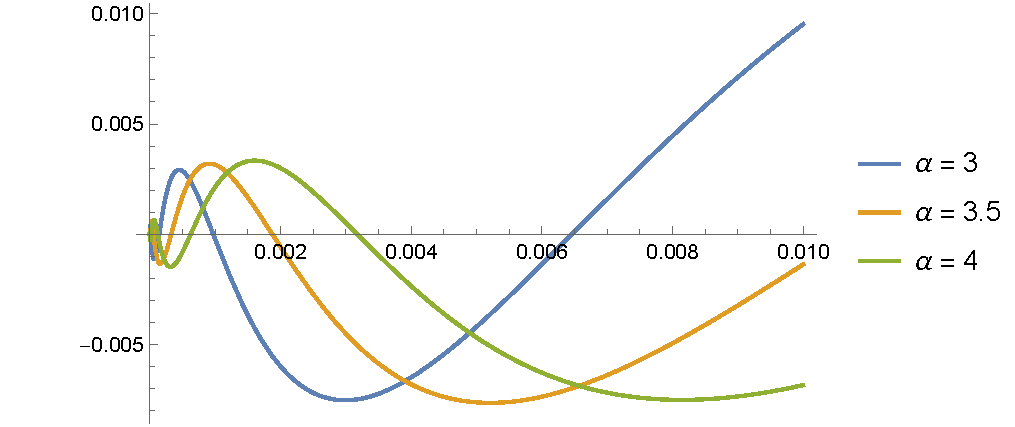
\includegraphics[width=0.8\linewidth]{bessel.pdf}
    \caption{The $\sqrt{x} K_{ig} (\rho x)$ function, $\rho = 1$.} % qua serve caption
    \label{fig:bessel}
\end{figure}

The plot shows the oscillatory behavior of the function near the origin, which is the effect of the sinusoidal dependence on $g \ln(x)$.

It can be shown that the solution has an infinite number of zero crossings, regardless of its energy. Therefore, if the number of zero crossings corresponds to the number of solutions with lower energy, it implies that there's no ground state because it would have $-\infty$ energy, coherent to what we concluded from the scale invariance. \footnote{This observation is consistent with the variational principle.}

\vspace{4mm}
\noindent
Comparing this result to the previous Section~\ref{section:generic_potentials}, in this case, the same behavior occurs as for $s > 2$ (in the old notation), meaning the particle \textit{falls} towards the origin.

\subsection*{Conclusion}
We have showed that the $-a/x^2$ potential has no ground state, no matter the value of $a$, but we have already some differences.
Remembering that $\alpha = 2ma/\hbar^2$, if $\alpha<1/4$, negative energy states (\textit{i.e. bound states}) are not allowed, else if $\alpha > 1/4$, negative energy states are allowed but not quantized (every negative energy is admissible).

\vspace{4mm}
\noindent
It is important to note that the result for $\alpha < 1/4$ will be shown to be incorrect by the end of Section~\ref{section:xsqared_halfaxis}. Even if we don't know it yet, this highlights the consequences of the problem being described by a non self-adjoint Hamiltonian.
